
\documentclass[12pt]{article} % use larger type; default would be 10pt


\usepackage{graphicx}
\usepackage{framed}


%------------------------------------------------------%
% http://www.psychwiki.com/wiki/Analyzing_Data
% http://www.upa.pdx.edu/IOA/newsom/semclass/ho_missing.pdf
% http://www.uvm.edu/~dhowell/StatPages/More_Stuff/Missing_Data/Missing.html
% http://www.uvm.edu/~dhowell/StatPages/More_Stuff/Missing_Data/Missing.html
% http://www.stat.columbia.edu/~gelman/arm/missing.pdf
% https://onlinecourses.science.psu.edu/stat505/node/78
% http://rer.sagepub.com/content/45/4/543.full.pdf
% http://www.kdnuggets.com/faq/precision-recall.html

%------------------------------------------------------%
\title{Advanced Data Modeling - Week 12}
\author{Kevin O'Brien}

\begin{document}
\maketitle
\tableofcontents
\newpage
%---------------------------------------------------------------------%
\section{Classification}
\subsection{What Is Classification}
classification is the problem of identifying to which of a set of categories (sub-populations) a new observation belongs, on the basis of a training set of data containing observations (or instances) whose category membership is known.
Discriminant analysis is an example of a \textbf{classification} method.

% It assumes that different classes generate data based on different Gaussian distributions.

\begin{itemize}
\item To train (create) a classifier, the fitting function estimates the parameters of a Gaussian distribution for each class.
\item To predict the classes of new data, the trained classifier finds the class with the smallest misclassification cost.
\end{itemize}
%-----------------------------------------------------------------------------------%
%\subsection{Recall and Precision}
%
%In a classification task, the precision for a class is the number of true positives (i.e. the number of items correctly labeled as belonging to the positive class) divided by the total number of elements labeled as belonging to the positive class (i.e. the sum of true positives and false positives, which are items incorrectly labeled as belonging to the class). Recall in this context is defined as the number of true positives divided by the total number of elements that actually belong to the positive class (i.e. the sum of true positives and false negatives, which are items which were not labeled as belonging to the positive class but should have been).



%-----------------------------------------------------------------------%
\subsection{Types I and II Error}
A type I error is the incorrect rejection of a true null hypothesis.
A type II error is the failure to reject a false null hypothesis.
A type I error is a false positive. Usually a type I error leads one to conclude that a thing
or relationship exists when really it doesn't.
A type II error is a false negative.
\begin{tabular}{|c|c|c|}
  \hline
  % after \\: \hline or \cline{col1-col2} \cline{col3-col4} ...

& Null hypothesis ($H_0$) is true	& Null hypothesis ($H_0$) is false\\ \hline
Reject  & Type I error          & Correct outcome \\
null hypothesis 			& False positive	& True positive\\ \hline
Fail to reject 	&Correct outcome&Type II error\\
null hypothesis & True negative	& False negative\\
  \hline
\end{tabular}
%-----------------------------------------------------------------------%
\subsection{False Positive and False Negative error}

A false positive error, commonly called a ``false alarm" is a result that indicates a
given condition has been fulfilled, when it actually has not been fulfilled.
A false positive error is a \textbf{Type I error} where the test is checking a single condition,
and results in an affirmative or negative decision usually designated as "true or false".

A false negative error is where a test result indicates that a condition failed, while it actually was successful.
A false negative error is a \textbf{Type II error} occurring in test steps where a single
condition is checked for and the result can either be positive or negative.


\subsection{Confusion Matrix}

A \textbf{confusion matrix}, is a table with two rows and two columns that reports the number of false positives, false negatives, true positives, and true negatives.

This allows more detailed analysis than mere proportion of correct guesses (accuracy). Accuracy is not a reliable metric for the real performance of a classifier, because it will yield misleading results if the data set is unbalanced (that is, when the number of samples in different classes vary greatly).

For example, if there were 95 cats and only 5 dogs in the data set, the classifier could easily be biased into classifying all the samples as cats. The overall accuracy would be 95\%, but  in practice the classifier would have a 100\% recognition rate for the cat class but a 0\% recognition rate for the dog class.

%-------------------------------------------------------------------------------------%

\subsection{Sensitivity and Specificity}

Sensitivity and specificity are measures of the performance of a binary classification test.

\begin{itemize}
\item Sensitivity (also called the true positive rate, or the \textbf{recall} rate) measures the proportion of actual positives which are correctly identified as such (e.g. the percentage of sick people who are correctly identified as having the condition).
    \[ \mbox{sensitivity (Recall)} = \frac{ \mbox{number of true positives} } {\mbox{number of true positives} + \mbox{number of false negatives}} \]

\item Specificity measures the proportion of negatives which are correctly identified as such (e.g. the percentage of healthy people who are correctly identified as not having the condition, sometimes called the true negative rate).
    \[ \mbox{ Specificity} = \frac{ \mbox{number of true negatives} } {\mbox{number of false positives} + \mbox{number of true negatives}} \]

\end{itemize}

(Remark: We will use the terms \textbf{Sensitivity} and \textbf{Recall} interchangeably. Sensitivity is more commonly used in a medical context, while recall is more commonly used in data science.)

\subsection{Receiver Operating Characteristic (ROC) curve }


In a Receiver Operating Characteristic (ROC) curve the true positive rate (Sensitivity) is plotted in function of the false positive rate (100-Specificity) for different cut-off points. Each point on the ROC curve represents a sensitivity/specificity pair corresponding to a particular decision threshold. A test with perfect discrimination (no overlap in the two distributions) has a ROC curve that passes through the upper left corner (100\% sensitivity, 100\% specificity). Therefore the closer the ROC curve is to the upper left corner, the higher the overall accuracy of the test (Zweig and Campbell, 1993).

\begin{figure}
	\centering
	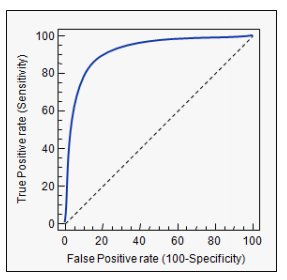
\includegraphics[width=0.7\linewidth]{ROCcurve}
	\caption{}
	\label{fig:roccurve}
\end{figure}

%----------------------------------------------------------------------------------%
\subsection{Properties of ROC Curves}
% ROC Curves
% Specificity and Sensitivity
An ROC curve demonstrates several things:
\begin{enumerate}
	\item It shows the tradeoff between sensitivity and specificity (any increase in sensitivity will be accompanied by a decrease in specificity).
	\item The closer the curve follows the upper-left border of the ROC space, the more accurate the test.
	\item The closer the curve comes to the 45-degree diagonal of the ROC space, the less accurate the test.
	\item The slope of the tangent line at a cutpoint gives the likelihood ratio (LR) for that value of the test.
	\item The area under the curve is a measure of accuracy.
\end{enumerate}
\end{document}